
%(BEGIN_QUESTION)
% Copyright 2010, Tony R. Kuphaldt, released under the Creative Commons Attribution License (v 1.0)
% This means you may do almost anything with this work of mine, so long as you give me proper credit

A new H1 Fieldbus segment seems to have a problem, and you suspect one of the Fieldbus cable conductors has become grounded.  A diagram of the system appears here:

$$\includegraphics[width=15.5cm]{i04596x01.eps}$$

Identify the diagnostic value of each of the following tests in determining whether or not a conductor has become grounded in this operating network segment.  If the measurement is a good test, mark it as ``Indicative.''  If the measurement tells you nothing about the state of the conductor, mark it as ``Indeterminate.''

% No blank lines allowed between lines of an \halign structure!
% I use comments (%) instead, so that TeX doesn't choke.

$$\vbox{\offinterlineskip
\halign{\strut
\vrule \quad\hfil # \ \hfil & 
\vrule \quad\hfil # \ \hfil & 
\vrule \quad\hfil # \ \hfil \vrule \cr
\noalign{\hrule}
%
% First row
{\bf Measurement} & {\bf Indicative} & {\bf Indeterminate} \cr
%
\noalign{\hrule}
%
% Another row
AC current between chassis ground and TB43-27 &  &  \cr
%
\noalign{\hrule}
%
% Another row
DC voltage between TB43-24 and TB43-25 &  &  \cr
%
\noalign{\hrule}
%
% Another row
AC voltage between TB105-2 and TB105-5 &  &  \cr
%
\noalign{\hrule}
%
% Another row
AC voltage between TB102-7 and TB102-9  &  &  \cr
%
\noalign{\hrule}
%
% Another row
AC voltage between TB102-4 and TB102-5  &  &  \cr
%
\noalign{\hrule}
%
% Another row
AC voltage between TB105-8 and TB105-9  &  &  \cr
%
\noalign{\hrule}
%
% Another row
Resistance between TB102-1 and TB102-2  &  &  \cr
%
\noalign{\hrule}
} % End of \halign 
}$$ % End of \vbox

For each of the ``Indicative'' measurements, specify what value of measurement would positively indicate a grounded conductor.

\vskip 20pt \vbox{\hrule \hbox{\strut \vrule{} {\bf Suggestions for Socratic discussion} \vrule} \hrule}

\begin{itemize}
\item{} An assumption being made here is that the multimeter is highly discriminating between AC and DC voltage values.  Is there a way you can test your own DMM to see how well it discriminates between AC and DC voltage?
\item{} Suppose a you measured a strong Fieldbus signal (700 mV) between terminal TB102-2 and earth ground.  Where could the ground fault be to cause this signal measurement?
\item{} Suppose a you measured a weak Fieldbus signal (5 mV) between terminal TB105-1 and earth ground.  Where could the ground fault be to cause this signal measurement?
\end{itemize}

\underbar{file i04596}
%(END_QUESTION)





%(BEGIN_ANSWER)

% No blank lines allowed between lines of an \halign structure!
% I use comments (%) instead, so that TeX doesn't choke.

$$\vbox{\offinterlineskip
\halign{\strut
\vrule \quad\hfil # \ \hfil & 
\vrule \quad\hfil # \ \hfil & 
\vrule \quad\hfil # \ \hfil \vrule \cr
\noalign{\hrule}
%
% First row
{\bf Measurement} & {\bf Indicative} & {\bf Indeterminate} \cr
%
\noalign{\hrule}
%
% Another row
AC current between chassis ground and TB43-27 &  & $\surd$ \cr
%
\noalign{\hrule}
%
% Another row
DC voltage between TB43-24 and TB43-25 &  & $\surd$ \cr
%
\noalign{\hrule}
%
% Another row
AC voltage between TB105-2 and TB105-5 &  & $\surd$ \cr
%
\noalign{\hrule}
%
% Another row
AC voltage between TB102-7 and TB102-9  & $\surd$ &  \cr
%
\noalign{\hrule}
%
% Another row
AC voltage between TB102-4 and TB102-5  &  & $\surd$ \cr
%
\noalign{\hrule}
%
% Another row
AC voltage between TB105-8 and TB105-9  & $\surd$ &  \cr
%
\noalign{\hrule}
%
% Another row
Resistance between TB102-1 and TB102-2  &  & $\surd$ \cr
%
\noalign{\hrule}
} % End of \halign 
}$$ % End of \vbox

If when measuring AC voltage between TB102-7 and TB102-9, you detect 0 volts, it means the positive conductor is grounded.  If measuring between the same two points you detect full FF signal voltage, it means the negative conductor is grounded.

\vskip 10pt

If when measuring AC voltage between TB105-8 and TB105-9, you detect 0 volts, it means the negative conductor is grounded.  If measuring between the same two points you detect full FF signal voltage, it means the positive conductor is grounded.

%(END_ANSWER)





%(BEGIN_NOTES)


%INDEX% Fieldbus, FOUNDATION (H1): segment troubleshooting

%(END_NOTES)

